\part{Développer une fonctionnalité d'évaluation : proposer un vue synthétique des performances d'un modèle de transcription Lectaurep dans une application avec Python et l'API Kraken}\label{partie_3}

Si dans la partie 2 nous oartions d'un existant, la mission présenter ici plus expérimental. Cependatn même dans le dev RD on part rarement de la page blanche sous section 1).
Le but était de dev une application permettant dd [issue]
-> établir des métriques
-> modéliser 
-> conception 
-> perspectives et des idées pour la suite des dévellopements 
-> premiers tests avec des transcription Lectaurep et premiers retours sur la plateforme avec d'autres utilisateurs 

\chapter{État de l'art pour l'évaluation des modèles de transcription entraînés avec le système HTR Kraken}

\section{Banc d'essai des outils existants : limites et avantages}

Avant de nous penché sur le dévellopement de l'outil Kraken-Benchmark, nous avons fait un état des lieux des soultions existantes pour évaluer 

Parmis les conclusions 

\section{Les métriques pour évaluer la transcription en question : définitions et recherche}

reprendre mémoire alix pour CER WER
comparer la transcription GT et revient à comparer deux chaines de caractères
Parmi les métriques retenus pour comparer des chaines de caractères 2 catégories similarité sémantique et syntxique (defs)
-> rappel des métriques
-> essai de métriques : concevoir des visualisations originales 
-> voir jupyter notebook
Un modèle d’HTR est entraîné sur des données d’apprentissage, c’est-à-dire des transcriptions manuelles vérifiées qui servent de ground truth ou « vérité terrain », auxquelles on compare les résultats de la reconnaissance automatique et sur la base desquelles ont effectue des corrections. Les performances d’un modèle sont évaluées par la comparaison entre les résultats
de l’HTR et une ground truth (vérité terrain, une transcription manuelle vérifiée et
certifiée comme correcte) : on calcule le Character Error Rate (CER) et le Word Error
Rate (WER), c’est-à-dire le taux d’erreurs concernant les caractères et celui concernant
les mots, en prenant en compte les trois types d’erreurs : les caractères mal reconnus,
ceux qui sont absents et ceux qui sont introduits dans les résultats de l’HTR sans être effectivement présents


\chapter{Le développement d'une application : Kraken-Benchmark}

\section{Modèlisation}

use case idéal

\subsection{envitonnement datascience}
-> schéma
-> IDE Pycharm
-> stack packages et choix

\section{Conception et usages}

\newpage
\begin{figure}
    \centering
    \centerline{\fbox{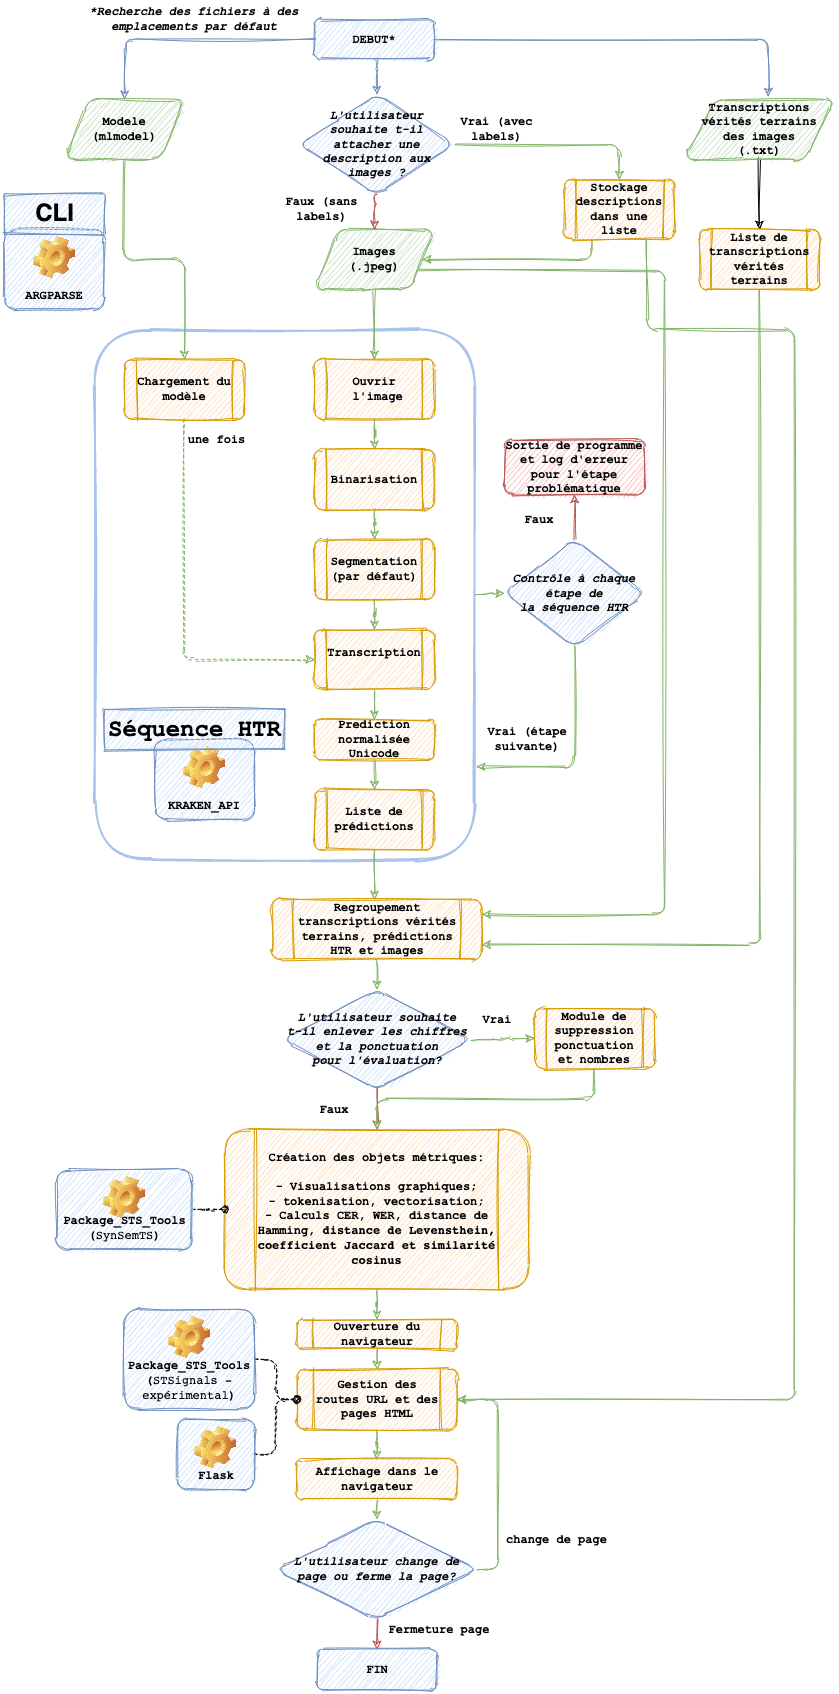
\includegraphics[width=17cm, height=22.5cm]{Kraken-Benchmark_modelisation.png}}}
    \caption{Algorigramme de Kraken-Benchmark.   \textcopyright L. Terriel, 2020, Diagrams.net}
    \label{fig:generateur_tei}
\end{figure}
suvi de projet

-> CVS Gitlab itération 
-> Code review / pairring 
-> Pylint -> 
-> au début Jinja puis Flask 
-> POO pour la librairie => avantages
-> Jules Verne Tests 
-> re
-> fonctionnement et usages / fonctionnalités 
-> retour de florianne 
\section{Perspectives d'amélioration pour l'application}
-> manque tests unitaires : projet interne au labo 
-> CLI plus user-friendly 
-> relier informations du format pivot XML TEI dans Kraken-Benchmark 

\chapter{Tests de Kraken-Benchmark sur les images de répertoires de notaires}
\section{Préparation du corpus et mise en place des tests}
\section{Déroulement et résultats des tests}
\section{Un bilan mitigé ? des propositions pour améliorer les scores}

Les ré
reprendre mémoire alix pour CER WER Transkribus

-> Les modèles utilisés présenté des problèmes sous entrainement et sur entrainement



Globalement les problèmes sur des données plus nombreuses et mixtes. Initialement le random set (700) devait être entièrement trasncrits 
pour permettre des entrainements sur des variétés de répertoire nombreux et entrainer un modèle général. Ce qui permettra d'atteindre des accuracy plus intéréssants et finetuner des modèles pour certains types de notaires. 
la variabilité des écritures obstacle dans la reconnaissance ex. ecritures très sérrés
Cependant l'approche actuel du DMC consiste à transcrire notaire par notaire (Riant, puis Dufour Marotte), pour des questions de facilité pour les annotateurs du projet LEctaurep, à partir du golden set. Conséquences : 1) fournis des données centrés sur un notaire et 2) pas assez nombreuses 3) rend compte de résultats toujours très faibles. 

Alix a entrainé récémment des modèles qui pourront être tester sur qui expose ces difficultés (graphiques Alix et résultats) mais ces nouveaux modèles n'ont pas encore testés dans KBapp

=> il faut donc attendre encore un plus grands nombres d'annotations pour exploiter ce random set et fournir des données plus nombreuses et variés. 



-> correcteur automatique
-> mieux formalisés les conventions de transcription des vérités terrains pour disposer de données d'entraînement plus efficaces
-> 
-> key word sppoting pour tenter la (Marie Laurence Bonhomme)

%POUR METTRE 4 PETITES IMAGES COTE À COTE

\begin{figure}[h] %CHAQUE MINIPAGE EST UNE IMAGE
    \begin{minipage}[c]{.46\linewidth} %ÇA TU TOUCHES PAS
        \centering
%        \includegraphics{} %LA TU MET L'IMAGE ET SI TU VEUX RÉGLER LA TAILLE TU MET LES [width et height] AVANT LES {}
    \end{minipage}
    \hfill%
    \begin{minipage}[c]{.46\linewidth}
        \centering
 %       \includegraphics{}
    \end{minipage}
    \hfill%
        \begin{minipage}[c]{.46\linewidth}
        \centering
 %       \includegraphics{}
    \end{minipage}
    \hfill%
        \begin{minipage}[c]{.46\linewidth}
        \centering
   %     \includegraphics{}
    \end{minipage}
    \caption{BLABLA} %ET TU METS LA LÉGENDE ICI
\end{figure}
% MERCI QUI!?... B-)